\setcounter{mtc}{5} %indique le numéro réel du chapitre, pour la mini table des matières
\chapter{Project Overview}
\minitoc  %insert la minitoc

\graphicspath{{Chapitre1/figures/}}
%==============================================================================
\pagestyle{fancy}
\fancyhf{}
\fancyhead[R]{\bfseries\chaptername~\thechapter. }
\fancyfoot[R]{\thepage}
\renewcommand{\headrulewidth}{0.5pt}
\renewcommand{\footrulewidth}{0pt}
%\renewcommand{\chaptermark}[1]{\markright{\MakeUppercase{\chaptername~\thechapter. #1 }}{}}
%\renewcommand{\sectionmark}[1]{\markright{\thechapter.\thesection~ #1}}

\begin{spacing}{1.2}
%==============================================================================

\section*{Introduction}
This opening chapter establishes the foundation of the graduation project by introducing the
host company and defining the project’s scope. We examine the organizational context,
outline the main objectives and challenges, and present the methodological framework that
guides the development process.


\section{Host Company: Google} 

\subsection{Presentation} 
Founded in 1998, Google LLC is a global leader in technology and innovation. As a subsidiary of Alphabet Inc., Google’s mission is to organize the world’s information and make it universally accessible and useful. Guided by values such as innovation, accessibility, sustainability, and user trust, Google has established itself as one of the most influential companies shaping the digital era. Its culture emphasizes collaboration, diversity, inclusion, and impact-driven engineering, enabling continuous leadership in research and product development.

\begin{figure}[!ht]\centering

\includegraphics[scale=0.07]{Images/google_logo.png}
\caption{Google Logo}
\label{fig:google_logo}
\end{figure}

\subsection{Products and services} 
Google offers a broad ecosystem of products and services that touch nearly every aspect of digital life. Among its flagship consumer products are Google Search, Maps, Gmail, Chrome, and the Android operating system, serving billions of users daily. 

Beyond consumer services, Google develops enterprise and cloud-based solutions such as Google Cloud Platform and Google Workspace, as well as advanced AI systems like Vertex AI. The company also invests in hardware, including Pixel devices, Nest smart home products, and ChromeOS. 

These products reflect Google’s commitment to connecting people, improving productivity, and driving digital transformation worldwide.

\begin{figure}[!ht]\centering
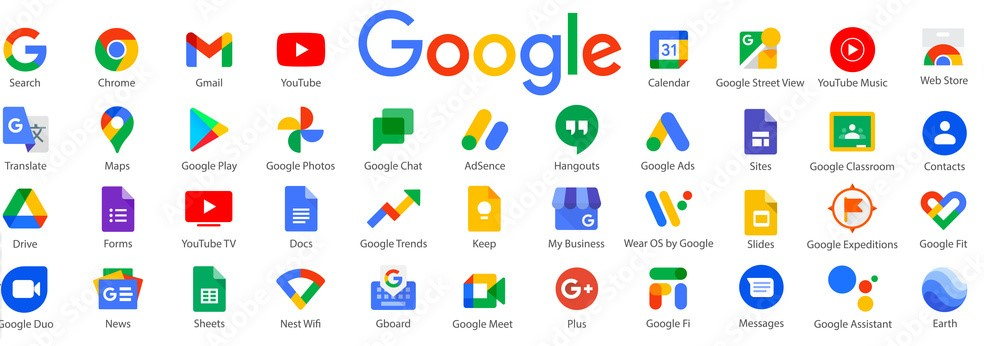
\includegraphics[scale=1.1]{Images/google_products.jpg}
\caption{Overview of some Google products}
\label{fig:google_products}
\end{figure}

\subsection{Focus Area} 
\subsubsection{YouTube}
Acquired by Google in 2006, YouTube has become the world’s leading video-sharing platform, serving more than two billion logged-in users monthly. It empowers individuals to create, share, and discover video content globally while sustaining a vibrant creator economy. From a technical perspective, YouTube integrates video processing, recommendation systems, live streaming, advertising, and trust and safety to deliver a seamless experience across devices.

\begin{figure}[!ht]\centering

\includegraphics[scale=0.07]{Images/youtube_logo.png}
\caption{YouTube Logo}
\label{fig:youtube_logo}
\end{figure}

\subsubsection{YouTube Developer Infrastructure Team}
Within YouTube’s engineering organization, the Developer Infrastructure (Dev Infra) team supports thousands of engineers building the platform. The team develops tooling, automation, and guidelines that improve efficiency, reliability, and consistency in software development. By maintaining developer velocity and quality at scale, the Dev Infra team contributes directly to YouTube’s ability to innovate and grow.




\section{Project Overview}

\subsection{Project Context}
This project was developed within the scope of my host team YoutTube Dev Infra, which focuses on supporting developers by providing tools and extensions that improve their day-to-day workflows. As part of this mission, the team is exploring how artificial intelligence can be leveraged to further assist developers. One concrete idea is to enhance their existing extension by introducing a feature that helps enforce internal best practices. The goal is to explore how large language models (LLMs) can complement traditional approaches, offering developers more intelligent and context-aware guidance directly within the IDE.

In addition, this project is carried out as part of the National Institute of Applied Science and Technology’s fifth-year mandatory final project, which is required to obtain the software engineering degree.

\subsection{Existing Solutions}
To support best practices and maintain code quality, teams currently rely on three main approaches:
\begin{itemize}
    \item \textbf{Code Reviews:} Engineers provide human feedback on design, readability, and best practices during review sessions. Recently, AI-assisted reviews have also been introduced, helping both reviewers and developers by suggesting improvements.
    
    \item \textbf{Presubmit Checks:} Automated checks executed before code is submitted. These ensure correctness, style consistency, and prevent simple errors.
    
    \item \textbf{Rule-Based Checks (Work in Progress):} Tools under development to enforce simple, objective rules such as naming conventions or syntax. These checks are intended for measurable guidelines and provide consistent, automated verification.
\end{itemize}

Together, these mechanisms form the current framework supporting developers in maintaining quality and consistency across the codebase.

\subsection{Problem Statement}
While these approaches provide valuable support, they also leave significant gaps in practice.  
\begin{itemize}
    \item \textbf{Delayed Feedback:} The most meaningful guidance on design and best practices typically arrives during code reviews, after development is complete. This often requires rework and slows iteration.  
    \item \textbf{Limited Scope of Presubmit Checks:} Presubmits focus on correctness and safety rather than nuanced best practices, leaving developers without proactive guidance in those areas.  
    \item \textbf{Surface-Level Coverage of Rule-Based Checks:} Rule-based tools can only enforce simple, objective rules. They are not able to reason about context-dependent or subjective best practices.  
\end{itemize}

As a result, developers lack timely, intelligent support during the actual coding phase, where guidance would be most efficient and impactful.  

\subsection{Proposed Solution}
This project introduces an \textbf{AI-assisted feedback system integrated directly into the coding workflow}.  
\begin{itemize}
    \item \textbf{Real-Time Guidance:} Provide developers with immediate, context-aware suggestions while they are writing code.  
    \item \textbf{Framework-Specific Best Practice Enforcement:} Go beyond syntax and correctness by surfacing adherence to YouTube’s internal framework guidelines early in the development process.  
    \item \textbf{Reduced Review Burden:} Shift part of the best practice enforcement from manual reviews to the authoring stage, making reviews faster and more focused on higher-level insights.  
\end{itemize}

By bringing intelligent, framework-aware feedback closer to the point of coding, the solution aims to reduce back-and-forth during reviews, ensure internal consistency, and accelerate development velocity.

\section{Work Methodology}

\subsection{Agile Development Approach}
Agile practices were adopted to support iterative development and maintain flexibility in responding to evolving requirements. This approach allowed continuous integration of feedback from the host and co-host, ensuring that each increment of work aligned with both technical goals and the broader product vision. Testing, validation, and code reviews were incorporated throughout the process to maintain high quality, while frequent collaboration provided clarity and shared ownership of outcomes. Agile principles also complemented Google’s focus on engineering excellence, including rigorous design reviews, thorough testing, robust code reviews, and DevOps-enabled automation.

\subsection{Kanban Workflow}
The dynamic workload of the YouTube Developer Infrastructure (Dev Infra) team, including feature requests, bug fixes, and maintenance tasks, was managed using a Kanban workflow. By visualizing tasks and limiting work in progress, the team could prevent bottlenecks and quickly shift focus to urgent issues when necessary. Work was structured into stages to maintain clear coordination while allowing the flexibility to adapt priorities as requirements evolved.  

The Kanban workflow included the following stages:

\begin{itemize}
    \item \textbf{Backlog:} Prioritized collection of feature requests, enhancements, and bug fixes.
    \item \textbf{Research \& Design:} Assessment of technical feasibility and preparation of design specifications.
    \item \textbf{Development:} Implementation and integration of features into the system.
    \item \textbf{Review \& Testing:} Code review, unit tests, and integration tests to ensure quality and correctness.
    \item \textbf{Deployment:} Release of validated features to developer environments.
\end{itemize}

\begin{figure}[H]
    \centering
    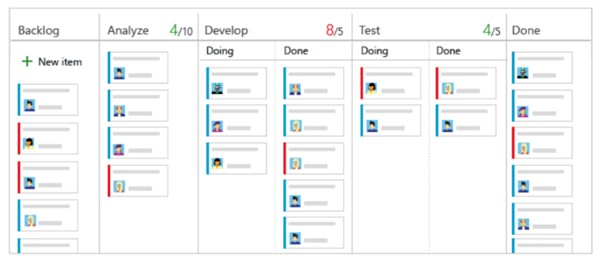
\includegraphics[scale=0.9]{Images/kanban_workflow.jpg}
    \caption{Kanban Workflow}
    \label{fig:kanban_workflow}
\end{figure}


\subsection{Development Process}
The project followed an iterative engineering cycle designed to balance thorough planning with incremental delivery. Each stage was supported by structured practices, dedicated tools, and regular collaboration:

\begin{itemize}
    \item \textbf{Ideation and Research:} The project began with an exploration phase to clarify objectives, gather requirements, and investigate potential solution directions. This stage combined independent research with collaborative discussions to assess feasibility and align on priorities.
    
    \item \textbf{Design and Planning:} A detailed design document was authored to present the technical choices, architectural considerations, and proposed workflow. This document was reviewed by engineers, iteratively refined, and approved. The final work plan was then transferred to the internal task management system, enabling structured tracking and prioritization.
    
    \item \textbf{Implementation:} Development was performed in small, reviewable increments using Google’s internal development environment within the company-wide repository. Each change was submitted accompanied by unit tests, and validated through both manual and AI-assisted code reviews. The implementation combined Python for backend logic, RPCs for inter-service communication, and TypeScript for the frontend.
    
    \item \textbf{Testing and Validation:} Functionality and reliability were verified continuously. Automated unit tests ensured correctness at the component level, while integration reviews validated the behavior within the larger system.
    
    \item \textbf{Maintenance and Optimization:} Refactoring, bug fixes, and updates were performed throughout development, particularly as some dependencies evolved or methods became deprecated. This ensured that the solution remained consistent, maintainable, and aligned with evolving standards.
\end{itemize}

Collaboration was supported through a structured communication rhythm, combining regular syncs with the host and co-host, weekly team meetings, and occasional cross-team discussions. This cadence provided timely feedback, clear guidance, and alignment on shared dependencies.

\begin{figure}[H]
    \centering
    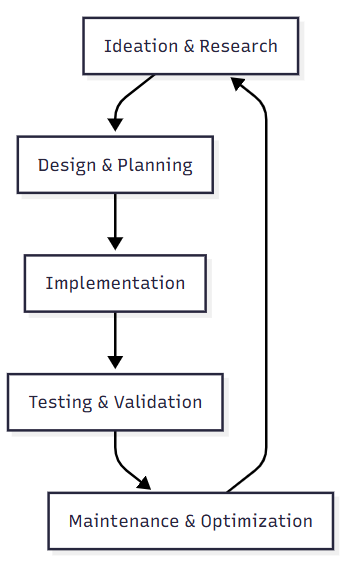
\includegraphics[scale=0.8]{Images/dev_process.png}
    \caption{Project Development Iteration Cycle}
    \label{fig:development_cycle}
\end{figure}

\subsection{Project Timeline}
The project spanned four months (May 5 – September 5, 2025). Work was scheduled based on business priorities and technical dependencies. Early weeks focused on research and design, followed by implementation, testing, and iterative refinement.

% Landscape page for timeline
\newpage
\begin{landscape}
\vspace*{\fill}
\begin{figure}[!ht]
    \centering
    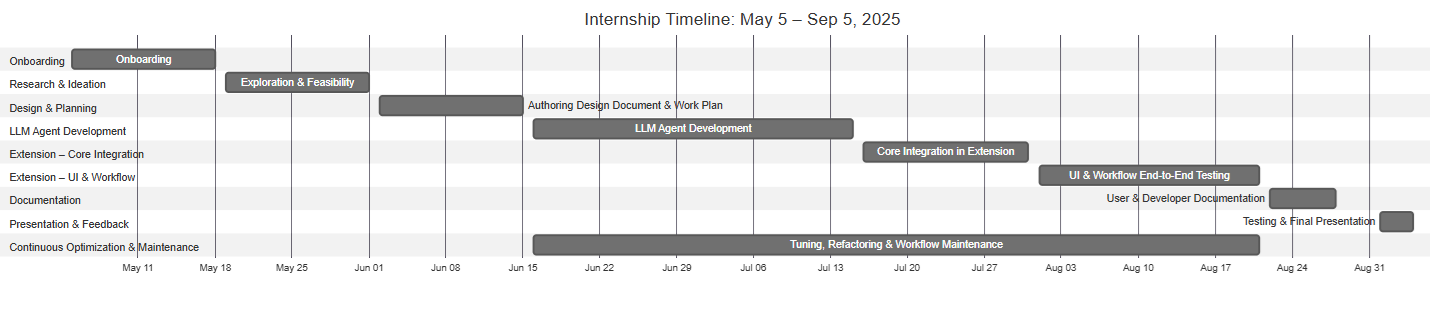
\includegraphics[width=1.3\textwidth,height=0.9\textheight,keepaspectratio]{Images/project_timeline.png}
    \caption{Project Timeline - Detailed Schedule}
    \label{fig:project_timeline}
\end{figure}
\vspace*{\fill}
\end{landscape}
\newpage


\section*{Conclusion}
In summary, this chapter outlined the project’s context by presenting the host company, defining the problem, and clarifying the main objectives and challenges. It also described the methodology chosen to guide the work, which provides the basis for the technical developments detailed in the following chapters.



%==============================================================================
\end{spacing}
